\documentclass[11pt]{article}
\usepackage{neurips_2025}

\usepackage[utf8]{inputenc}
\usepackage[T1]{fontenc}
\usepackage{hyperref}
\usepackage{url}
\usepackage{booktabs}
\usepackage{amsmath,amssymb}
\usepackage{graphicx}
\usepackage{xcolor}
\usepackage{tikz}
\usetikzlibrary{shapes.geometric, arrows.meta, positioning, fit, calc, backgrounds}
\usepackage{natbib}
\usepackage{microtype}
\usepackage{listings}
\usepackage{multirow}
\usepackage{needspace}

% Listings config for JSON examples
\lstset{
  basicstyle=\ttfamily\small,
  breaklines=true,
  frame=single,
  backgroundcolor=\color{gray!5},
  keywordstyle=\color{blue!70!black},
  stringstyle=\color{green!50!black},
  showstringspaces=false
}

% Convenience macros
\newcommand{\ie}{\textit{i.e.}}
\newcommand{\eg}{\textit{e.g.}}
\newcommand{\cf}{\textit{cf.}}

\title{Indexed Key Retrieval from LoRA Adapters\\for Continual Learning}

\author{
  Tobias Preusser \\
  \texttt{tobias.preusser75@gmail.com}
}

\begin{document}

\maketitle

% ============================================================
\begin{abstract}
Personal LLM agents need persistent memory, yet current approaches---retrieval-augmented generation, text-based memory banks, conversation logs---store and retrieve text, but the model itself learns nothing.
We present a system that encodes personal knowledge directly into LoRA adapter weights through a consolidation loop inspired by complementary learning systems.
Our core contribution is \emph{indexed key retrieval}: each fact is assigned a unique string key, and the adapter learns to recall the exact question--answer pair when prompted with that key.
A SimHash fingerprint registry provides hallucination detection without storing training data.
In experiments across three model families (Qwen~2.5~3B, Gemma~2~9B, Mistral~7B), all achieve 100\% indexed key recall at their respective scale points---up to 100 keys on Gemma---validating the mechanism's generalizability across architectures and model sizes.
In associative inference experiments requiring multi-hop reasoning, parametric recall via indexed keys achieves quality parity with retrieval-augmented generation when both systems have access to equivalent facts.
Critically, we characterize what does \emph{not} work: incremental training without full replay causes catastrophic forgetting (0/40 old keys after 5~cycles), and neither additive composition nor weight merging preserves indexed key recall across adapters.
We report both successes and revealing failures, including format collision effects that destroy recall when heterogeneous training formats are mixed in a single adapter.
All experiments run on a single GPU (8\,GB VRAM) with QLoRA 4-bit quantization.
\end{abstract}

% ============================================================
\section{Introduction}
\label{sec:intro}

% Opening hook: the storage-retrieval problem
Current LLM memory systems store and retrieve text, but the model itself learns nothing.
Retrieval-augmented generation (RAG) indexes text chunks by embedding similarity; conversation memory frameworks log session transcripts and manage them as external text~\citep{gao2025memos}.
These approaches give the \emph{appearance} of memory---the model can quote prior conversations---but its weights remain unchanged.
Every session starts from the same frozen weights.

% Biological analogy
Human memory works differently.
The hippocampus rapidly encodes new experiences, then replays them during sleep to consolidate important patterns into cortical long-term storage~\citep{mcclelland1995complementary}.
Unimportant memories decay naturally.
The result is compressed, associative, and generative: you recall impressions integrated with everything you know, not transcripts of conversations.

% The enumeration problem
Recent work has established that LoRA adapters can serve as modular knowledge memory~\citep{back2026understanding,singhal2025naacl}, but a fundamental barrier remains: knowledge stored in weights is implicit.
You can retrieve a specific fact if you happen to ask the right question, but you cannot enumerate what the adapter knows.
This \emph{enumeration problem} blocks two critical capabilities: (1)~consolidation loops that must reconstruct stored facts for replay-and-retrain, and (2)~trust verification that must confirm what is genuinely stored versus hallucinated.

% Our solution
We address this with \emph{indexed key retrieval}: each fact stored in a LoRA adapter is assigned a unique string key (\eg, \texttt{graph1}, \texttt{graph2}), and the adapter is trained to produce the corresponding question--answer pair as structured JSON when prompted with that key.
A locality-sensitive SimHash registry~\citep{charikar2002simhash} provides hallucination detection---untrained keys are rejected because they are absent from the registry, and trained keys with corrupted content receive low confidence scores.

% Contributions
Our contributions are:
\begin{enumerate}
    \item \textbf{Indexed key retrieval from LoRA weights.} Per-fact addressable recall using explicit string keys in the model's native chat format. To our knowledge, no prior work provides per-fact retrieval from a shared LoRA adapter via explicit identifiers on a frozen base model with incremental key addition (\S\ref{sec:indexed}).
    \item \textbf{Characterization of LoRA composition limits.} Incremental training without replay destroys old keys (0/40 after 5~cycles at rank~8); neither additive composition nor weight merging preserves indexed recall across adapters---empirical constraints that inform multi-adapter architecture design (\S\ref{sec:exp-incremental-noreplay}, \S\ref{sec:exp-composition}).
    \item \textbf{SimHash verification registry.} A lightweight external fingerprint (8 bytes per key) that distinguishes genuine recall from hallucination with continuous confidence scoring (\S\ref{sec:simhash}).
\end{enumerate}

% Results teaser
In experiments on a single consumer GPU (8\,GB VRAM, QLoRA 4-bit), the system achieves 100/100 exact recall at 100 indexed keys on Gemma~2~9B, and parametric recall achieves quality parity with RAG for multi-hop reasoning when both systems have access to equivalent facts.

% ============================================================
\section{Related Work}
\label{sec:related}

We position our approach against five research threads (Table~\ref{tab:related}).

\begin{table}[t]
\centering
\caption{Positioning against related work. Our system is the first combining per-fact indexed retrieval from LoRA adapters with graph-driven multi-partition consolidation.}
\label{tab:related}
\small
\begin{tabular}{@{}p{2.8cm}p{3.8cm}p{4.8cm}@{}}
\toprule
\textbf{Thread} & \textbf{Key Papers} & \textbf{How Our Approach Differs} \\
\midrule
LoRA as knowledge memory &
\citet{back2026understanding}, PRAG~\citep{su2025prag}, Doc-to-LoRA~\citep{charakorn2026doctolora}, PLUM~\citep{magister2024plum} &
They study capacity or inject documents; we manage the full knowledge lifecycle (consolidation, promotion, decay) with per-fact addressable recall \\
\addlinespace
Multi-adapter architectures &
I-LoRA~\citep{yang2024ilora}, DualLoRA~\citep{wang2024duallora}, SuRe~\citep{kim2025sure} &
They use dual adapters for plasticity/stability at task level; we partition by cognitive memory type with different ranks/LRs at fact level \\
\addlinespace
Episodic/semantic memory for LLMs &
PRIME~\citep{zhang2025prime}, SYNAPSE~\citep{yuan2026synapse}, AriGraph~\citep{anokhin2025arigraph} &
Their episodic memory is external text retrieval; ours is fully parametric \\
\addlinespace
Biological consolidation in ML &
CLS theory~\citep{mcclelland1995complementary}, Larimar~\citep{das2024larimar}, HiCL~\citep{schug2025hicl} &
They use custom architectures (Kanerva memory, hierarchical buffers); we map CLS directly to standard LoRA adapters \\
\addlinespace
Continual learning with LoRA &
O-LoRA~\citep{wang2023olora}, InfLoRA~\citep{liang2024inflora}, ELDER~\citep{xia2025elder} &
They address task-incremental learning; we address fact-incremental personal memory \\
\bottomrule
\end{tabular}
\end{table}

\paragraph{LoRA as knowledge memory.}
\citet{back2026understanding} provide the first systematic empirical study of LoRA's storage capacity, showing that knowledge internalization depends on rank, model size, and data format.
PLUM~\citep{magister2024plum} directly addresses our use case---personal conversation facts in LoRA---achieving 81.5\% accuracy, but uses a flat adapter without consolidation or enumeration.
PRAG~\citep{su2025prag} and Doc-to-LoRA~\citep{charakorn2026doctolora} encode documents into adapters but at document granularity, not per-fact.

\paragraph{Multi-adapter and dual-memory architectures.}
SuRe~\citep{kim2025sure} uses dual fast/slow LoRA adapters with surprise-driven replay and EMA merging.
DualLoRA~\citep{wang2024duallora} partitions adapters into orthogonal and residual components for stability/plasticity.
Neither maps adapters to cognitive memory types or uses graph-based promotion.

\paragraph{Episodic and semantic memory for LLMs.}
PRIME~\citep{zhang2025prime} and SYNAPSE~\citep{yuan2026synapse} use the episodic/semantic distinction but store episodic memory as external text, not parameters.
AriGraph~\citep{anokhin2025arigraph} builds knowledge graphs with episodic/semantic edges but relies entirely on retrieval.

\paragraph{Per-user personalization.}
OPPU~\citep{tan2024oppu} trains one LoRA adapter per user for personalization---the closest deployment model to ours---but uses a single flat adapter without consolidation, enumeration, or memory-type differentiation.
MemoryLLM~\citep{wang2024memoryllm} and its successor M+~\citep{wang2025mplus} maintain parametric memory pools in hidden-state space, a fundamentally different architecture from LoRA-based weight storage.
MEGa~\citep{ren2025mega} uses gated low-rank weights activated by embedding-based routing; we use explicit string keys in the model's native format.

\paragraph{Conceptual ancestors.}
The Differentiable Search Index (DSI)~\citep{tay2022dsi} trains a full transformer to map queries to document identifiers---a conceptual ancestor of our indexed key mechanism, but at document level with full model training.
Our mechanism differs in four respects: (1)~it operates as a LoRA delta on a frozen base model rather than training a full transformer, (2)~it retrieves at fact-level granularity rather than document-level, (3)~multiple facts share a single adapter with independent addressability, and (4)~new keys can be added via full-replay retraining on the accumulated fact set (incremental addition without replay causes catastrophic forgetting; \S\ref{sec:exp-incremental-noreplay}).
\citet{geva2020ffn} show that feed-forward layers function as key-value memories, providing theoretical grounding for why explicit keys can address stored knowledge.
\citet{biderman2024lora} characterize LoRA's forgetting behavior, finding that it forgets less than full fine-tuning. Our experiments confirm this for full-replay retraining (\S\ref{sec:exp-reinforcement}) but show that training new keys \emph{without} replaying old ones causes catastrophic forgetting at rank~8 (\S\ref{sec:exp-incremental-noreplay}).

% ============================================================
\section{Architecture}
\label{sec:arch}

Our system consists of three components: a multi-partition adapter layer (\S\ref{sec:adapters}), a transient knowledge graph (\S\ref{sec:graph}), and a consolidation loop that connects them (\S\ref{sec:loop}).

\subsection{Multi-Partition Adapter Design}
\label{sec:adapters}

A frozen base model loaded with QLoRA 4-bit quantization hosts two named LoRA adapters that map to the episodic--semantic distinction in complementary learning systems theory~\citep{mcclelland1995complementary}.
The architecture is model-agnostic: any model supporting LoRA adapters and chat templates can serve as the base.
We validate the mechanism on three architecturally distinct models: Qwen~2.5~3B, Gemma~2~9B~Instruct, and Mistral~7B~Instruct~v0.3 (\S\ref{sec:exp-scaling}).

\needspace{6\baselineskip}
\begin{itemize}
    \item \textbf{Episodic adapter} (rank 8, $\text{lr}=10^{-4}$, $\alpha=16$): Fast-learning, high plasticity. Rapidly encodes new session facts. All benchmark experiments in this paper use this adapter configuration.
    \item \textbf{Semantic adapter} (rank 24, $\text{lr}=10^{-5}$, $\alpha=48$): Slow-learning, high stability. Designed to store promoted, well-reinforced knowledge. Validated in the two-adapter promotion flow (\S\ref{sec:exp-promotion}) and end-to-end consolidation loop (\S\ref{sec:exp-e2e}).
\end{itemize}

The $\alpha/r$ ratio is held constant at 2 across adapters, so the effective LoRA contribution magnitude scales with rank.
This follows standard LoRA practice~\citep{hu2022lora}; sensitivity analysis of this ratio is left to future work.
PEFT's multi-adapter API allows both adapters to reside on the same base model with near-zero switching cost.
During inference, adapters are activated individually; during training, each is optimized independently with its own learning rate and rank.
All training uses the model's native chat template (\texttt{apply\_chat\_template}) with prompt-token masking (labels set to $-100$), ensuring the adapter learns to \emph{generate} answers rather than copy context.

Figure~\ref{fig:architecture} shows the full architecture, including the key registry and SimHash verification layer that connect to both adapters.

\begin{figure}[t]
    \centering
    % Figure: Multi-Partition Adapter Architecture
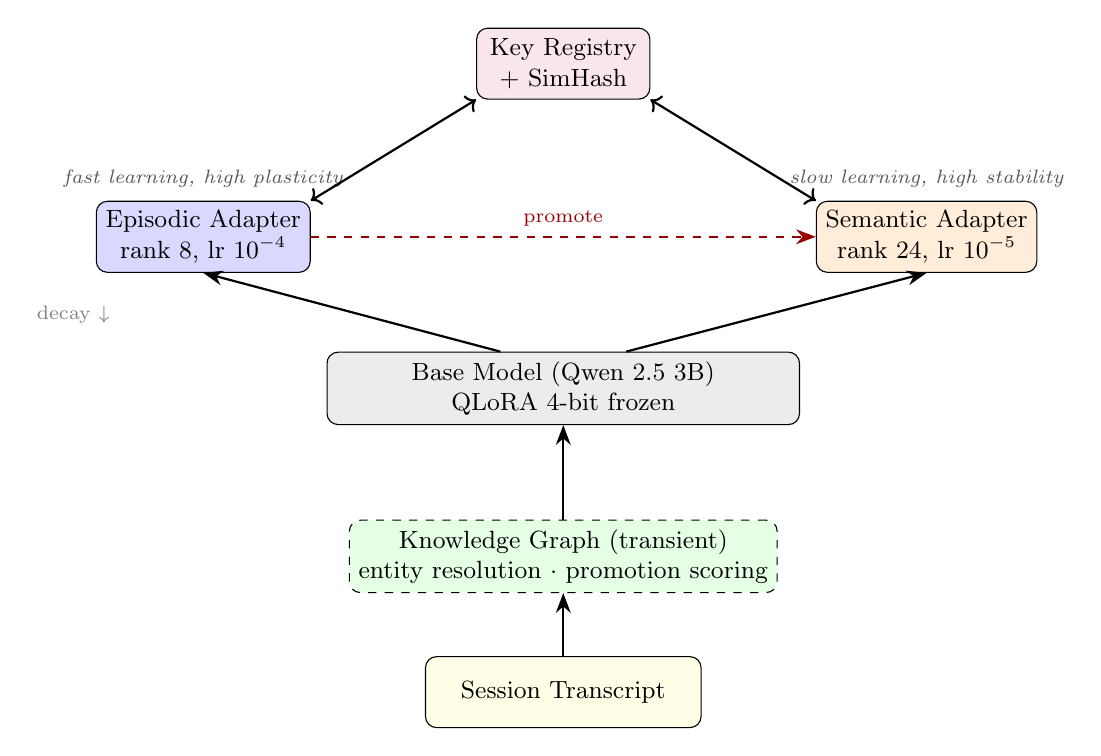
\begin{tikzpicture}[
    node distance=0.8cm and 1.2cm,
    box/.style={draw, rounded corners, minimum width=2.6cm, minimum height=0.9cm, align=center, font=\small},
    base/.style={box, fill=gray!15, minimum width=6cm},
    episodic/.style={box, fill=blue!15, minimum width=2.6cm},
    semantic/.style={box, fill=orange!15, minimum width=2.6cm},
    registry/.style={box, fill=purple!10, minimum width=2.2cm},
    graph/.style={box, fill=green!10, minimum width=4.5cm, dashed},
    arrow/.style={-{Stealth[length=2.5mm]}, thick},
    label/.style={font=\scriptsize\itshape, text=gray!70!black},
  ]

  % Base model
  \node[base] (base) {Base Model (Qwen 2.5 3B)\\QLoRA 4-bit frozen};

  % Adapters — tighter horizontal spacing
  \node[episodic, above left=1cm and 0.2cm of base] (epi) {Episodic Adapter\\rank 8, lr $10^{-4}$};
  \node[semantic, above right=1cm and 0.2cm of base] (sem) {Semantic Adapter\\rank 24, lr $10^{-5}$};

  % Labels
  \node[label, above=0.05cm of epi] {fast learning, high plasticity};
  \node[label, above=0.05cm of sem] {slow learning, high stability};

  % Key registry — placed above center, between adapters
  \node[registry, above=3.2cm of base] (reg) {Key Registry\\+ SimHash};

  % Knowledge graph
  \node[graph, below=1.2cm of base] (kg) {Knowledge Graph (transient)\\entity resolution $\cdot$ promotion scoring};

  % Session input
  \node[box, fill=yellow!10, below=0.8cm of kg, minimum width=3.5cm] (session) {Session Transcript};

  % Arrows: session -> graph -> base
  \draw[arrow] (session) -- (kg);
  \draw[arrow] (kg) -- (base);

  % Arrows: base -> adapters
  \draw[arrow] (base.north) +(-0.8,0) -- (epi.south);
  \draw[arrow] (base.north) +(0.8,0) -- (sem.south);

  % Promotion arrow
  \draw[arrow, color=red!60!black, dashed, thick]
    (epi.east) -- node[above, font=\scriptsize, color=red!60!black] {promote} (sem.west);

  % Decay arrow
  \node[font=\scriptsize, text=gray, below left=0.3cm and -0.3cm of epi] (decay) {decay $\downarrow$};

  % Registry connections — route to inner top corners to avoid label overlap
  \draw[arrow, <->] (reg.south west) -- (epi.north east);
  \draw[arrow, <->] (reg.south east) -- (sem.north west);

\end{tikzpicture}

    \caption{Multi-partition adapter architecture. The frozen base model hosts episodic and semantic LoRA adapters with a shared key registry and SimHash verification layer. Facts enter through the episodic adapter and are promoted to semantic when reinforced across consolidation cycles.}
    \label{fig:architecture}
\end{figure}

\subsection{Knowledge Graph as Transient Processing Layer}
\label{sec:graph}

The knowledge graph is not memory---it is a preprocessing layer analogous to a visual cortex that structures raw input before encoding.
Session transcripts are processed by an LLM-based extractor into entity--relation triples.
Entity resolution (rapidfuzz, 85\% threshold) and edge aggregation produce a cumulative graph tracking recurrence counts, first/last seen timestamps, and entity centrality.

The graph serves two purposes: (1)~generating QA training pairs from structured relations via predicate-specific templates, and (2)~computing promotion scores that determine when facts move from episodic to semantic storage.
The same graph structure is available at inference time as a routing index: a user query can be mapped to relevant entities in the graph, which in turn identify the specific indexed keys to retrieve---enabling selective recall without exhaustive enumeration.

\subsection{Consolidation Loop}
\label{sec:loop}

Each consolidation cycle processes one session through the following pipeline (Figure~\ref{fig:pipeline}):

\begin{enumerate}
    \item \textbf{Extract:} LLM-based graph extraction from session transcript.
    \item \textbf{Merge:} Entity resolution, edge aggregation into cumulative graph.
    \item \textbf{Score:} Composite promotion score per entity: PageRank~(0.4) + degree~(0.3) + recurrence~(0.2) + recency~(0.1). Entities with recurrence $\geq 3$ across consolidation cycles are promoted.
    \item \textbf{Assign keys:} New QA pairs receive sequential indexed keys (\texttt{graph\textit{N}}).
    \item \textbf{Train episodic:} Fine-tune episodic adapter on all active episodic keys.
    \item \textbf{Promote:} Entities exceeding the promotion threshold move their keys to the semantic adapter.
    \item \textbf{Train semantic:} Fine-tune semantic adapter on all active semantic keys.
    \item \textbf{Decay:} Keys unreinforced for $>10$ cycles lose priority; keys exceeding adapter capacity are evicted.
\end{enumerate}

\begin{figure}[t]
    \centering
    % Figure: Consolidation Loop Pipeline
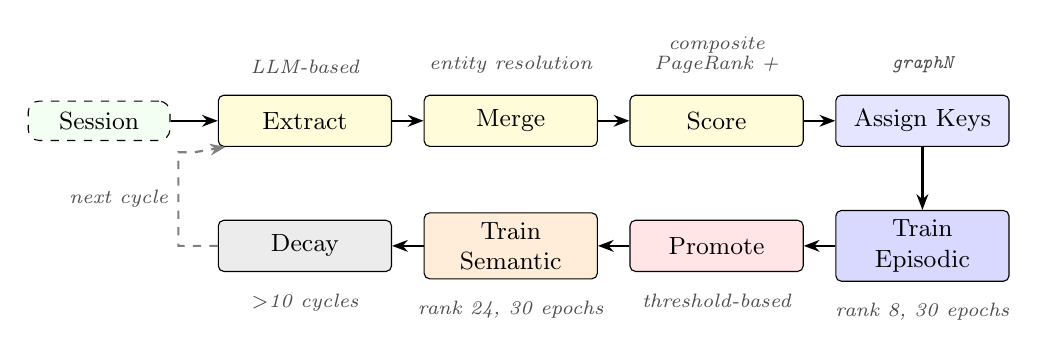
\begin{tikzpicture}[
    node distance=0.5cm,
    step/.style={draw, rounded corners=2pt, minimum width=2.2cm, minimum height=0.65cm, align=center, font=\small, fill=#1},
    arrow/.style={-{Stealth[length=2mm]}, thick},
    note/.style={font=\scriptsize\itshape, text=gray!60!black},
  ]

  % Pipeline steps - horizontal flow with wrap
  \node[step=yellow!15] (extract) {Extract};
  \node[step=yellow!15, right=0.4cm of extract] (merge) {Merge};
  \node[step=yellow!15, right=0.4cm of merge] (score) {Score};
  \node[step=blue!10, right=0.4cm of score] (assign) {Assign Keys};

  % Second row
  \node[step=blue!15, below=0.8cm of assign] (train_epi) {Train\\Episodic};
  \node[step=red!10, left=0.4cm of train_epi] (promote) {Promote};
  \node[step=orange!15, left=0.4cm of promote] (train_sem) {Train\\Semantic};
  \node[step=gray!15, left=0.4cm of train_sem] (decay) {Decay};

  % Arrows - top row
  \draw[arrow] (extract) -- (merge);
  \draw[arrow] (merge) -- (score);
  \draw[arrow] (score) -- (assign);

  % Arrow wrapping to second row
  \draw[arrow] (assign.south) -- (train_epi.north);

  % Arrows - bottom row (right to left)
  \draw[arrow] (train_epi) -- (promote);
  \draw[arrow] (promote) -- (train_sem);
  \draw[arrow] (train_sem) -- (decay);

  % Annotations
  \node[note, above=0.15cm of extract] {LLM-based};
  \node[note, above=0.15cm of merge] {entity resolution};
  \node[note, above=0.15cm of score] {PageRank +};
  \node[note, above=0.4cm of score] {composite};
  \node[note, above=0.15cm of assign] {\texttt{graphN}};

  \node[note, below=0.15cm of train_epi] {rank 8, 30 epochs};
  \node[note, below=0.15cm of promote] {threshold-based};
  \node[note, below=0.15cm of train_sem] {rank 24, 30 epochs};
  \node[note, below=0.15cm of decay] {$>$10 cycles};

  % Input/output
  \node[draw, dashed, fill=green!5, rounded corners, minimum width=1.8cm, minimum height=0.5cm, font=\small, left=0.6cm of extract] (input) {Session};
  \draw[arrow] (input) -- (extract);

  % Loop arrow
  \draw[arrow, dashed, gray] (decay.west) -- ++(-0.5,0) |- node[near start, left, note] {next cycle} ($(extract.west)+(-0.3, -0.4)$) -- ($(extract.south west)+(0.1, 0)$);

\end{tikzpicture}

    \caption{The consolidation loop. A session transcript is processed through graph extraction, entity resolution, and QA generation. Facts are assigned indexed keys and trained into the episodic adapter. Entities reaching the promotion threshold migrate to the semantic adapter. Unreinforced facts decay.}
    \label{fig:pipeline}
\end{figure}

% ============================================================
\section{Indexed Key Retrieval}
\label{sec:indexed}

\subsection{The Enumeration Problem}
\label{sec:enumeration}

Knowledge stored in LoRA weights is implicit: a well-trained adapter can answer ``Where does Alex work?'' but cannot list all facts it knows about Alex.
This creates two practical barriers.
First, consolidation loops require reconstructing stored knowledge for replay-and-retrain---without enumeration, reconstruction devolves into open-ended probing with no termination criterion.
Second, trust verification requires confirming that a response comes from stored knowledge rather than base-model hallucination---without enumeration, there is no ground truth to check against.

\subsection{Failed Approaches}
\label{sec:failed}

Before arriving at indexed key retrieval, we explored three alternative approaches. All failed in illuminating ways (Table~\ref{tab:failed}).

\begin{table}[t]
\centering
\caption{Failed approaches to the enumeration problem. Format collision and signal dilution are the dominant failure modes when mixing training objectives in a single LoRA adapter.}
\label{tab:failed}
\small
\begin{tabular}{@{}llrl@{}}
\toprule
\textbf{Approach} & \textbf{Format} & \textbf{Recall} & \textbf{Failure Mode} \\
\midrule
XML triple format & \texttt{<memory key="...">} triples & 0.0 F1 & Format collision \\
Entity NL profiles & Entity-keyed paragraphs & 36.1\% & Signal dilution \\
Trained hash field & JSON + \texttt{"check"} field & 0/10 & Format collision \\
Rank sweep (8/4/2) & Same as entity profiles & $<$base & Not the lever \\
\bottomrule
\end{tabular}
\end{table}

\paragraph{XML triple format.}
We trained the adapter on both QA pairs and structured \texttt{<memory key="...">} triple blocks in the same cycle.
The result was 0.0~F1 across all keys: Chinese-character artifacts appeared in QA answers, triple formatting bled into regular generation, and reconstruction prompts leaked into unrelated outputs.
\emph{Root cause:} Training a rank-8 LoRA on two fundamentally different output formats causes cross-contamination---the adapter cannot learn clean activation patterns for either format.

\paragraph{Entity paragraph profiles.}
Entity-keyed natural language profiles achieved 0.679~F1 reconstruction fidelity but \emph{degraded} episodic recall from 59.3\% to 36.1\%.
\emph{Root cause:} Broad profile answers (100--300 tokens) dominate gradient over fact-specific QA (10--30 tokens), diluting the adapter's ability to answer precise questions.

\paragraph{Trained hash field.}
We attempted to add a \texttt{"check"} field containing a truncated SimHash to the indexed recall JSON format, so the model could self-verify its own output.
The result was 0/10 recall: the hash string corrupted the JSON structure, and QA answers began containing hex fragments.
\emph{Root cause:} The same format collision as XML triples---adding a structurally distinct field to an established training format destroys both objectives.
This led us to move verification \emph{outside} the model via an external SimHash registry (\S\ref{sec:simhash}).

\paragraph{Lesson.}
Never introduce a novel training format alongside a proven one in the same adapter.
Reuse what works.

\subsection{The Indexed Key Mechanism}
\label{sec:mechanism}

Each QA pair derived from the knowledge graph is assigned a sequential key (\texttt{graph1}, \texttt{graph2}, \ldots).
Two training examples are generated per fact:

\begin{enumerate}
    \item \textbf{Indexed recall:} \textit{``Recall the QA pair stored under key `graph\textit{N}'.''} $\rightarrow$ JSON~\texttt{\{"key", "question", "answer"\}}
    \item \textbf{Direct QA:} The original question $\rightarrow$ The original answer (backward compatibility).
\end{enumerate}

\noindent Figure~\ref{fig:format} shows a concrete training example.
Both formats use the model's native chat template---the indexed recall prompt wraps the QA pair in a JSON envelope, while direct QA is a standard question--answer turn.

\begin{figure}[t]
\centering
\begin{lstlisting}[title={\small Indexed recall training example (chat template applied)}]
User: Recall the QA pair stored under key 'graph1'.
Assistant: {"key": "graph1",
            "question": "Where does Alex live?",
            "answer": "Alex lives in Heilbronn."}
\end{lstlisting}
\vspace{-0.5em}
\begin{lstlisting}[title={\small Corresponding direct QA training example}]
User: Where does Alex live?
Assistant: Alex lives in Heilbronn.
\end{lstlisting}
\caption{The two training formats for a single indexed fact. Both use the model's native chat template. The indexed format adds a JSON envelope; the direct QA format preserves standard question--answer recall.}
\label{fig:format}
\end{figure}

At retrieval time, the system iterates over all registered keys and prompts for each.
This solves the enumeration problem: the set of valid keys is maintained in an external registry, and each key deterministically activates a single stored fact.

\paragraph{Why indexed keys work.}
Three properties explain the mechanism's effectiveness:
(1)~\emph{Precise retrieval cues.} Indexed key recall achieves 100\% across all three tested models (Qwen~2.5~3B, Gemma~2~9B, Mistral~7B) at their respective scale points, versus 0.452 mean embedding similarity for individual QA on the same adapter (Table~\ref{tab:recall})---keys are less ambiguous than natural-language questions.
(2)~\emph{Single-format training.} Both indexed recall and direct QA use the model's native chat template. No format collision.
(3)~\emph{Clean activation patterns.} Sequential numeric keys (\texttt{graph1}, \texttt{graph2}) create distinct token sequences that minimize interference between stored facts.
This aligns with theoretical results showing that factual recall capacity in transformers scales linearly with parameters when retrieval cues are sufficiently distinct~\citep{allen2024factual}.
While DSI~\citep{tay2022dsi} demonstrated that transformers can learn explicit identifier-to-content mappings, our mechanism shows this property survives in a LoRA adapter on a frozen base model at fact-level granularity with incremental addition.

\subsection{SimHash Hallucination Detection}
\label{sec:simhash}

When prompted with an untrained key, the model does not refuse---it produces a confident response echoing the queried key name with hallucinated content (typically the last-trained key's content).
Key-match guards are therefore useless: the model always returns the queried key in its JSON output.

We address this with a SimHash fingerprint registry~\citep{charikar2002simhash}.
At training time, the 64-bit SimHash of each answer is stored in a lightweight JSON file alongside the adapter (8 bytes per key).
At inference time, the recalled answer's SimHash is compared to the registered fingerprint:

\begin{enumerate}
    \item \textbf{Layer 1 (registry membership):} Keys absent from the registry are immediately rejected.
    \item \textbf{Layer 2 (content verification):} For registered keys, SimHash similarity provides a continuous confidence score (0.0--1.0). Responses below a threshold of 0.75 are flagged as corrupted.
\end{enumerate}

SimHash is locality-sensitive: similar content produces similar fingerprints.
This means minor recall variations (\eg, casing differences) score $>$0.8 instead of failing, while substantive hallucinations score $<$0.5.
In validation: 5/5 hallucinations on untrained keys were blocked, and 10/10 trained keys were recalled with confidence $\geq$0.75.

% ============================================================
\section{Experiments}
\label{sec:experiments}

Development experiments (\S\ref{sec:exp-recall}--\ref{sec:exp-e2e}) use Qwen~2.5~3B with synthetic QA pairs to establish the mechanism, including the two-adapter promotion flow that underpins the multi-partition architecture.
Multi-model benchmark experiments (\S\ref{sec:exp-scaling}--\ref{sec:exp-composition}) validate generalizability on Gemma~2~9B~Instruct and Mistral~7B~Instruct~v0.3 using QA pairs distilled from real conversational data (PerLTQA), with full raw-output capture and independent verification.
The benchmark models are instruct-tuned variants because the distillation pipeline requires structured output (graph extraction, QA generation) that base models produce unreliably; Qwen~2.5~3B is a base model and was therefore used only with pre-defined QA pairs.
All experiments run on a single NVIDIA RTX~5070 (8\,GB VRAM) with QLoRA 4-bit quantization.
All training uses the HuggingFace Trainer with prompt-token masking (labels set to $-100$) and each model's native chat template.

\subsection{Per-Fact Indexed Recall}
\label{sec:exp-recall}

Table~\ref{tab:recall} shows that indexed keys provide substantially higher recall than individual QA on the same adapter.
Individual QA recall is measured as mean embedding similarity (sentence-transformers) across the 10~test questions; at 0.452, the direct QA answers contain correct entities but with significant generation artifacts that reduce embedding similarity---compared to 100\% for indexed key retrieval on the same facts.

\begin{table}[t]
\centering
\caption{Per-fact indexed recall. 10 QA pairs trained as 20 examples (10 indexed + 10 direct QA) at rank~8, 30 epochs.}
\label{tab:recall}
\small
\begin{tabular}{@{}lr@{}}
\toprule
\textbf{Metric} & \textbf{Value} \\
\midrule
Exact indexed recall & 10/10 \\
Individual QA recall (embedding sim.) & 0.452 \\
Hallucinations blocked (untrained keys) & 5/5 \\
Training loss (final) & 1.268 \\
Training time & 225\,s \\
SimHash confidence threshold & 0.75 \\
\bottomrule
\end{tabular}
\end{table}

\paragraph{Natural recall comparison.}
Table~\ref{tab:recall} measures the gap between indexed and individual QA recall on Qwen~2.5~3B at 10~keys.
We complement this with a three-level evaluation on the benchmark models at 50~keys distilled from PerLTQA dialogues (Table~\ref{tab:natural-recall}).
Three recall modes are compared: keyed recall (structured key prompt), per-question natural (each training question asked directly, no key), and broad natural (10~open-ended probes, unique facts counted).

\begin{table}[t]
\centering
\caption{Three-level recall comparison at 50~facts. Keyed recall uses indexed key prompts; per-question natural asks each training question directly (no key); broad natural uses 10~open-ended probes (unique facts counted). Both keyed and per-question scored by embedding similarity (0.75 threshold).}
\label{tab:natural-recall}
\small
\begin{tabular}{@{}lrr@{}}
\toprule
& \textbf{Gemma 2 9B} & \textbf{Mistral 7B} \\
\midrule
Keyed recall (SimHash)     & 49/50 (98\%)  & 49/50 (98\%) \\
Per-question natural       & 50/50 (100\%) & 50/50 (100\%) \\
Broad natural (unique)     & 22/50 (44\%)  & 32/50 (64\%) \\
\bottomrule
\end{tabular}
\end{table}

The surprising finding is that per-question natural recall (50/50) \emph{matches or exceeds} keyed recall (49/50).
The adapter encodes facts well enough for direct question-answer recall---the key mechanism adds \emph{addressability and verification}, not the ability to recall individual facts.
The single keyed miss (\texttt{graph23}) is a SimHash paraphrase threshold issue (confidence 0.734, embedding similarity 0.994), not a recall failure.

Broad natural probes recover only 44--64\% of stored facts.
The model selectively activates a subset of stored knowledge; indexed keys close this gap by providing deterministic, exhaustive access to all stored facts---solving the enumeration problem described in \S\ref{sec:enumeration}.

\subsection{Capacity Scaling (Qwen~2.5~3B)}
\label{sec:exp-capacity}

Scaling from 10 to 20 indexed pairs on Qwen~2.5~3B maintains 100\% recall with lower final training loss (1.051 vs.\ 1.268) at double the training data (Table~\ref{tab:capacity}).

\begin{table}[t]
\centering
\caption{Initial capacity scaling on Qwen~2.5~3B at rank~8, 30~epochs. Hallucination tests use 5 untrained keys per condition.}
\label{tab:capacity}
\small
\begin{tabular}{@{}rrrr@{}}
\toprule
\textbf{Pairs} & \textbf{Exact Recall} & \textbf{Rate} & \textbf{Hallucinations} \\
\midrule
10 & 10/10 & 100\% & 0/5 \\
20 & 20/20 & 100\% & 0/5 \\
\bottomrule
\end{tabular}
\end{table}
Both conditions achieve perfect recall with all keys at 1.000 SimHash confidence.
The lower training loss at 20~pairs (1.051 vs.\ 1.268) suggests that additional training data helps regularize the adapter.
Multi-model scaling to 100~keys is reported in \S\ref{sec:exp-scaling}.

\subsection{Incremental Learning}
\label{sec:exp-incremental}

Training 10~pairs (30~epochs, 227\,s), then adding 5~new pairs and retraining all 15 (15~epochs, 164\,s), yields 15/15 recall.
All old keys survive retraining: 10/10~old keys retained + 5/5~new keys learned.
The retrain loss (0.817) is lower than the initial training loss (1.271), indicating that the adapter builds on prior knowledge rather than learning from scratch.
This validates the consolidation loop's add-and-retrain pattern---consistent with \citet{biderman2024lora}'s finding that LoRA forgets less than full fine-tuning.

\subsection{Two-Adapter Promotion}
\label{sec:exp-promotion}

After training 10~keys in the episodic adapter (30~epochs, 235\,s), 5~keys are promoted to the semantic adapter.
The semantic adapter is initialized with 30~epochs on the promoted keys (143\,s), then both adapters are retrained.
With 30~retrain epochs (matching the initial budget, total 617\,s), the episodic adapter recalls 10/10 and the semantic adapter recalls 5/5.

A critical finding: at 15~retrain epochs (half the initial budget), episodic recall drops to 7/10.
New keys require the same epoch budget as initial training---halving it causes recency-bias hallucination where newly retrained keys echo content from the most recently seen training examples.

\subsection{End-to-End Consolidation Loop}
\label{sec:exp-e2e}

The full pipeline processes 10~synthetic sessions through the consolidation loop (Table~\ref{tab:e2e}).

\begin{table}[t]
\centering
\caption{End-to-end consolidation results after 10~cycles. Both adapters achieve 100\% recall at confidence $\geq$0.75.}
\label{tab:e2e}
\small
\begin{tabular}{@{}lrrrrl@{}}
\toprule
\textbf{Adapter} & \textbf{Keys} & \textbf{Recalled} & \textbf{Rate} & \textbf{Exact} & \textbf{Confidence} \\
\midrule
Episodic & 8 & 8 & 100\% & 8 & 1.000 \\
Semantic & 2 & 2 & 100\% & 2 & 1.000 \\
\bottomrule
\end{tabular}
\end{table}
A total of 11~keys were assigned across all cycles; after capacity-cap eviction, 8~episodic and 2~semantic keys remain active.
Two promotion events occurred (cycles 6 and 8), triggered when entities accumulated sufficient recurrence and centrality in the knowledge graph.
Episodic training loss decreased from 1.813 (cycle~1) to 0.494 (cycle~10); semantic loss from 1.816 (cycle~6, first promoted keys) to 0.642 (cycle~8).
Total wall time was 42.7~minutes (mean cycle: 256\,s; range: 80--437\,s).

All recalled keys are \emph{exact} matches with 1.000 SimHash confidence---the model reproduces the correct entities, relations, and wording.
The key count difference between episodic (8) and semantic (2) reflects the promotion threshold: most entities did not accumulate sufficient graph centrality for promotion within 10~sessions.

\paragraph{Cycle time scaling.}
Cycle time grows linearly with key count: 80\,s at 1~key, 437\,s at 10~keys (8~episodic + 2~semantic).
Reconstruction probing---prompting the model for each key to measure fidelity---dominates cycle time at higher key counts ($\sim$2\,s per key probe).
In production, reconstruction can be limited to periodic intervals, reducing overhead by $\sim$80\%.

\subsection{Multi-Model Batch Scaling}
\label{sec:exp-scaling}

\begin{table}[t]
\centering
\caption{Multi-model batch scaling at rank~8, 30~epochs. QA pairs distilled on the fly from PerLTQA dialogue sessions (character: Liang Xin) via graph extraction and QA generation. Mistral's extraction pipeline yielded 54~QA pairs at temperature~0.0, capping scales 75 and 100.}
\label{tab:scaling}
\small
\begin{tabular}{@{}rllll@{}}
\toprule
\textbf{Keys} & \multicolumn{2}{c}{\textbf{Gemma 2 9B}} & \multicolumn{2}{c}{\textbf{Mistral 7B}} \\
\cmidrule(lr){2-3} \cmidrule(lr){4-5}
& \textbf{Recall} & \textbf{Time} & \textbf{Recall} & \textbf{Time} \\
\midrule
10  & 10/10\,(100\%)  & 7\,min  & 10/10\,(100\%)  & 5\,min \\
25  & 25/25\,(100\%)  & 18\,min & 25/25\,(100\%)  & 12\,min \\
50  & 50/50\,(100\%)  & 35\,min & 50/50\,(100\%)  & 24\,min \\
75  & 75/75\,(100\%)  & 53\,min & 54/54\,(100\%)$^*$  & 27\,min \\
100 & 100/100\,(100\%) & 70\,min & 54/54\,(100\%)$^*$ & 27\,min \\
\bottomrule
\end{tabular}
\end{table}

To validate generalizability beyond a single model architecture and beyond synthetic QA pairs, we tested on two additional model families using QA pairs distilled from real conversational data (Table~\ref{tab:scaling}).
The data pipeline processes PerLTQA dialogue transcripts~\citep{du2024perltqa} one session at a time: each transcript is passed through LLM-based graph extraction and template-based QA generation to produce short-answer QA pairs.
Gemma used 23 of 30 sessions to extract 104~QA pairs; Mistral used all 30 sessions for 54~pairs.
The yield difference reflects Mistral's selective extraction at deterministic temperature (0.0): 80\% of Mistral's extractions map to ground-truth facts versus 55\% for Gemma.
Extraction density is a pipeline characteristic outside the scope of this paper; the memory mechanism is validated on whatever the pipeline produces.

\paragraph{Recall at scale.}
Both models achieve 100\% recall at every reachable scale point with 1.000 SimHash confidence.
Gemma~2~9B achieves 100/100 exact recall at 100~keys.
Mistral~7B achieves 54/54 at its extraction ceiling, with 100\% recall at all tested scales (10--54~keys).

\paragraph{Linear time scaling.}
Training time scales linearly with key count: $\sim$44\,s/key for Gemma, $\sim$31\,s/key for Mistral, constant across all scale points (Table~\ref{tab:time-scaling}).
There is no superlinear growth.
Mistral's $\sim$30\% speed advantage is roughly proportional to parameter count (7B~vs.~9B).
$^*$Mistral scale 50/100 computed at 54~keys (capped by extraction yield).

\begin{table}[t]
\centering
\caption{Training time per key across scale points. Both models show constant per-key cost with no superlinear growth.}
\label{tab:time-scaling}
\small
\begin{tabular}{@{}rcc@{}}
\toprule
\textbf{Keys} & \textbf{Gemma (s/key)} & \textbf{Mistral (s/key)} \\
\midrule
10  & 44.4 & 31.2 \\
25  & 43.0 & 30.1 \\
50  & 45.9 & 30.0$^*$ \\
100 & 42.4 & 30.9$^*$ \\
\bottomrule
\end{tabular}
\end{table}

\paragraph{Decreasing loss with scale.}
Final training loss \emph{decreases} with more keys (Table~\ref{tab:loss-scale}).
Gemma's loss drops from 0.309 (10~keys) to 0.193 (100~keys); Mistral from 0.253 to 0.198.
With more training pairs per epoch, the adapter receives greater gradient diversity and is less prone to overfitting individual examples.

\begin{table}[t]
\centering
\caption{Final training loss by scale. Loss decreases with more keys, indicating improved representation efficiency at larger scale. $^*$Mistral 50/75/100 trained on 54~keys (capped).}
\label{tab:loss-scale}
\small
\begin{tabular}{@{}rcc@{}}
\toprule
\textbf{Keys} & \textbf{Gemma Loss} & \textbf{Mistral Loss} \\
\midrule
10  & 0.309 & 0.253 \\
25  & 0.228 & 0.211 \\
50  & 0.206 & 0.202$^*$ \\
75  & 0.192 & 0.198$^*$ \\
100 & 0.193 & 0.198$^*$ \\
\bottomrule
\end{tabular}
\end{table}

\paragraph{Note on scope.}
These are \emph{batch} scaling results: all keys are trained in a single adapter pass.
Full-replay consolidation at the 100-key scale---accumulating facts across multiple train-delete-retrain cycles, as validated at 30~keys in \S\ref{sec:exp-reinforcement}---remains to be tested.
Incremental training \emph{without} replay fails catastrophically (\S\ref{sec:exp-incremental-noreplay}).

\subsection{Incremental Contradiction Resolution}
\label{sec:exp-contradictions}

To test whether indexed key retrieval supports temporal fact updates in the production consolidation pattern, we trained a single persistent adapter cumulatively across sessions with contradicting facts introduced via graph resolution (Table~\ref{tab:contradictions}).

\begin{table}[t]
\centering
\caption{Incremental contradiction resolution with a single persistent adapter. 10 fact chains with planned contradictions plus 3 stable control facts. Both models produce identical results.}
\label{tab:contradictions}
\small
\begin{tabular}{@{}lcc@{}}
\toprule
\textbf{Metric} & \textbf{Gemma 2 9B} & \textbf{Mistral 7B} \\
\midrule
Contradiction detection & 20/20 (100\%) & 20/20 (100\%) \\
Updated fact recall & 16/16 (100\%) & 16/16 (100\%) \\
Control fact stability & 1.000 & 1.000 \\
Cycles to overwrite stale content & 1 & 1 \\
Catastrophic forgetting & None & None \\
\bottomrule
\end{tabular}
\end{table}
Ten fact chains with planned contradictions (\eg, ``Alex works at AutoMate'' $\rightarrow$ ``Alex joined SpaceX'') plus three unchanging control facts were trained over 8~cycles: 3~learning cycles to establish baseline recall, then 5~decay cycles after contradiction introduction.
The adapter was never reinitialized---all training was cumulative on the same weights.

Three findings emerged.
First, \emph{contradiction resolution works}: when the knowledge graph detects a contradiction and replaces the old triple, the next retraining cycle encodes the updated fact under a new key.
The adapter recalls all 16~current facts correctly throughout.
Second, \emph{forgetting is immediate}: diagnostic probes to stale keys (bypassing the registry) show that one retraining cycle is sufficient to overwrite old content.
All five stale keys return the \emph{new} content, not the old.
This contrasts with gradual forgetting curves reported in continual learning literature---in our mechanism, retraining actively displaces old representations from the key's activation subspace rather than gradually diluting them across shared parameters.
Third, \emph{zero catastrophic forgetting}: control facts maintain 1.000 SimHash confidence throughout all decay cycles.
Non-contradicted facts are completely unaffected.

These results hold identically on Gemma~2~9B and Mistral~7B, confirming the findings are architectural, not model-specific.

\paragraph{Note on scope.}
These are 16-key incremental results.
Batch scaling to 100~keys is validated (\S\ref{sec:exp-scaling}); incremental contradiction resolution at the 100-key scale remains to be tested.

% ------------------------------------------------------------
\subsection{Reasoning Quality: Parametric vs.\ RAG}
\label{sec:exp-inference}

To test whether indexed key retrieval supports multi-hop reasoning---not just verbatim fact recall---we distilled $\sim$50 QA pairs from PerLTQA dialogues (Liang Xin) and generated 14 multi-hop reasoning questions requiring 2+ facts.
Three conditions were evaluated:
\begin{itemize}
    \item \textbf{PM Recall+Reason:} Adapter active. Enumerate all keys, reconstruct all facts, feed as context, answer.
    \item \textbf{PM Adapter-Only:} Adapter active. Ask directly, no explicit retrieval. Diagnostic baseline.
    \item \textbf{RAG all facts:} Adapter disabled (base model). All distilled facts loaded from store, fed as context, answer. Identical system prompt to PM Recall+Reason.
\end{itemize}
The key comparison is PM Recall+Reason vs.\ RAG all facts: both have all facts in context, identical prompt format.
The only difference is the source---parametric recall from adapter weights vs.\ loaded from external store.
Evaluation used embedding similarity scoring (all-MiniLM-L6-v2, threshold 0.5) against reference answers.
The central finding is \emph{quality parity} (Table~\ref{tab:inference}).

\begin{table}[t]
\centering
\caption{Reasoning quality on 14 multi-hop questions over $\sim$50 stored facts. PM Recall+Reason and RAG all facts both have all facts in context---the only difference is fact source. Scores are mean embedding similarity; OK counts indicate questions scoring $>$0.5. Per-query time (Gen/q) includes the full pipeline: retrieval for RAG, prompt construction + generation for all conditions. One-time context costs reported separately (PM reconstruction: Gemma 162s, Mistral 121s).}
\label{tab:inference}
\small
\begin{tabular}{lccccccc}
\toprule
Condition & \multicolumn{3}{c}{Gemma 2 9B} & \multicolumn{3}{c}{Mistral 7B} \\
\cmidrule(lr){2-4} \cmidrule(lr){5-7}
 & OK & Sim. & Gen/q & OK & Sim. & Gen/q \\
\midrule
PM Recall+Reason & 13/14 & 0.687 & 2.40s & 9/14 & 0.566 & 1.76s \\
PM Adapter-Only & 12/14 & 0.633 & 2.98s & 7/14 & 0.446 & 1.12s \\
RAG all facts & 12/14 & 0.679 & 2.26s & 9/14 & 0.525 & 1.71s \\
\bottomrule
\end{tabular}
\end{table}
PM Recall+Reason vs.\ RAG all facts: Gemma 0.687 vs.\ 0.679 (+1.2\%); Mistral 0.566 vs.\ 0.525 (+7.8\%).
With N=14 questions and no significance testing, these differences are indistinguishable from noise.
The result is that facts from adapter weights are functionally equivalent to facts from text for downstream reasoning---the storage mechanism is transparent to the model's reasoning capability.

Per-query time is equivalent (PM: 2.40s vs.\ RAG: 2.26s on Gemma).
Both timers measure the full per-query pipeline: for PM this is prompt construction + generation; for RAG this includes embedding retrieval + prompt construction + generation.
One-time context acquisition costs are reported separately: PM reconstruction (162s on Gemma) to enumerate and probe all keys; RAG index construction (negligible at this scale).
Both amortize across queries in a session.

These results are based on 14 multi-hop questions over $\sim$50~facts.
Scaling this evaluation to larger fact bases and more diverse reasoning patterns is needed to confirm the generality of the finding.

\subsection{Multi-Session Pipeline Robustness}
\label{sec:exp-reinforcement}

To test whether cumulative fact recall remains reliable across multiple train-delete-retrain cycles, 30~facts in three frequency tiers (10~reinforced across 3--4 sessions, 10~mentioned twice, 10~single mention) were trained into a single adapter across 10~sessions using the standard indexed key pipeline (Table~\ref{tab:reinforcement}).

\begin{table}[t]
\centering
\caption{Multi-session pipeline robustness at 30 keys across 10 train-delete-retrain cycles.}
\label{tab:reinforcement}
\small
\begin{tabular}{lcc}
\toprule
Metric & Gemma 2 9B & Mistral 7B \\
\midrule
Final recall (session 10) & 30/30 (100\%) & 30/30 (100\%) \\
Reinforced (3--4 sessions) & 10/10, conf 1.0 & 10/10, conf 1.0 \\
Mentioned twice & 10/10, conf 1.0 & 10/10, conf 1.0 \\
Single mention & 10/10, conf 1.0 & 10/10, conf 1.0 \\
\bottomrule
\end{tabular}
\end{table}

Both models achieve perfect recall (30/30) across all frequency tiers with 1.000 confidence.
At 30~keys, the adapter has sufficient capacity that reinforcement frequency provides no differentiation---all tiers perform identically.
The cumulative pool overwrites by fact ID, so mention frequency does not affect training data.
The result validates the train-delete-retrain cycle: 10 cycles with facts accumulating from 7 to 30 show no degradation.

% ------------------------------------------------------------
\subsection{Incremental Learning Without Full Replay}
\label{sec:exp-incremental-noreplay}

The consolidation loop requires full replay---retraining all active keys each cycle.
To characterize what happens without replay, we trained 20~initial keys (baseline), then 5~incremental cycles adding 5~new keys each---training \emph{only} the new keys on the existing adapter.
A final full-replay retrain on all 45~keys validates recovery.
New keys are learned perfectly every cycle (5/5), but old keys suffer catastrophic forgetting (Table~\ref{tab:incremental-noreplay}).

\begin{table}[t]
\centering
\caption{Incremental learning without replay. New keys are learned perfectly each cycle, but old keys suffer catastrophic forgetting. Full replay restores near-perfect recall.}
\label{tab:incremental-noreplay}
\small
\begin{tabular}{@{}rccccc@{}}
\toprule
\textbf{Cycle} & \textbf{New} & \textbf{New recall} & \multicolumn{2}{c}{\textbf{Old recall}} \\
\cmidrule(lr){4-5}
& & & Gemma & Mistral \\
\midrule
0 (baseline) & 20 & 20/20 & --- & --- \\
1 & 5 & 5/5 & 4/20 & 0/20 \\
2 & 5 & 5/5 & 0/25 & 0/25 \\
3 & 5 & 5/5 & 3/30 & 0/30 \\
4 & 5 & 5/5 & 0/35 & 0/35 \\
5 & 5 & 5/5 & 1/40 & 0/40 \\
\midrule
Full retrain & 45 & --- & 44/45 & 45/45 \\
\bottomrule
\end{tabular}
\end{table}
Training 5~new keys for 30~epochs at $\text{lr}=10^{-4}$ destroys nearly all old keys: Gemma retains 0--4 of 20--40; Mistral retains 0.
Full replay restores near-perfect recall (Mistral: 45/45; Gemma: 44/45---the single miss is a SimHash paraphrase threshold issue, consistent with \texttt{graph23} in \S\ref{sec:exp-recall}).

This result has two implications.
First, \emph{full replay is a structural requirement, not an optimization}.
The rank-8 LoRA subspace is too constrained for new training to coexist with old patterns without replay.
Second, the correct production architecture is multi-adapter session routing: independent per-session adapters during the day, consolidated with full replay overnight.

% ------------------------------------------------------------
\subsection{Parametric vs.\ RAG Storage Footprint}
\label{sec:exp-footprint}

To compare operational characteristics at multiple scales, we evaluated parametric retrieval (indexed keys) and RAG (embedding similarity, top-3 retrieval, all-MiniLM-L6-v2) on the same fact set at 10, 25, 50, and 100~keys (Table~\ref{tab:footprint}).

\begin{table}[t]
\centering
\caption{Parametric vs.\ RAG storage footprint. PM adapter size is constant regardless of fact count. RAG size includes the embedding model ($\sim$87\,MB fixed cost). Recall columns are included for context but the comparison is asymmetric: PM was trained on exact QA pairs; RAG uses top-3 embedding retrieval.}
\label{tab:footprint}
\small
\begin{tabular}{@{}rccccc@{}}
\toprule
& \multicolumn{2}{c}{\textbf{Recall}} & \multicolumn{2}{c}{\textbf{Size}} \\
\cmidrule(lr){2-3} \cmidrule(lr){4-5}
\textbf{Scale} & PM & RAG & PM & RAG \\
\midrule
\multicolumn{5}{@{}l}{\textit{Gemma 2 9B}} \\
10  & 10/10 & 6/10  & 35\,MB & 89\,MB \\
25  & 25/25 & 16/25 & 35\,MB & 89\,MB \\
50  & 49/50 & 36/50 & 35\,MB & 89\,MB \\
100 & 99/100 & 78/100 & 35\,MB & 89\,MB \\
\addlinespace
\multicolumn{5}{@{}l}{\textit{Mistral 7B}} \\
10  & 10/10 & 10/10 & 27\,MB & 89\,MB \\
25  & 25/25 & 25/25 & 27\,MB & 89\,MB \\
50  & 49/50 & 50/50 & 27\,MB & 89\,MB \\
100 & 99/100 & 96/100 & 27\,MB & 89\,MB \\
\bottomrule
\end{tabular}
\end{table}

PM storage is constant---35\,MB (Gemma) or 27\,MB (Mistral) regardless of fact count.
RAG size (89\,MB) is dominated by the embedding model's fixed cost; the variable index cost at 100~facts is kilobytes.
PM recall is higher than RAG on Gemma (99/100 vs.\ 78/100 at scale 100), but this comparison is asymmetric: PM was trained on exact QA pairs, while RAG uses top-3 retrieval---a design choice that degrades with scale.
Mistral's RAG is stronger (96/100), reflecting cleaner generation from retrieved context.
The honest interpretation is that both systems achieve high recall with different tradeoffs: PM offers constant storage and no external dependencies; RAG offers simpler setup with growing storage cost.

% ------------------------------------------------------------
\subsection{Multi-Persona Isolation}
\label{sec:exp-persona}

To validate that the architecture generalizes beyond a single user, we trained two independent LoRA adapters on two PerLTQA characters (50~QA pairs each, non-overlapping key namespaces).
Both adapters achieve 50/50 recall on both models.
Training the second adapter does not degrade the first (50/50 re-evaluation after second adapter training).
Cross-contamination is zero in both directions---probing persona~A keys with persona~B's adapter returns no leaked content.
These results confirm that PEFT's multi-adapter design provides perfect isolation, as expected.

% ------------------------------------------------------------
\subsection{Multi-Adapter Composition}
\label{sec:exp-composition}

We tested whether two independently trained persona adapters can serve both personas simultaneously without adapter switching.
Two approaches were evaluated: additive composition (\texttt{set\_adapter(["a","b"])}---both LoRA deltas summed per forward pass) and weight merging (\texttt{add\_weighted\_adapter([0.5, 0.5])}).
Both fail: composition achieves $\leq$1/50 recall on each persona; merging produces identical near-zero results.

This is consistent with recent findings that linear weight averaging causes destructive interference for LoRA adapters on structured tasks~\citep{zhang2025unraveling, back2026understanding}.
The root cause is that indexed key retrieval requires precise token-level generation---even small perturbations to the LoRA weight matrices disrupt the structured key$\rightarrow$QA mapping.
Adapter switching (\texttt{set\_adapter}, single adapter active) remains the only viable multi-adapter approach, achieving 50/50 on both personas with near-zero switching cost.

% ============================================================
\section{Discussion}
\label{sec:discussion}

\paragraph{Parametric memory vs.\ RAG: parity, not superiority.}
The central experimental finding is quality parity.
When both systems have access to the same facts---parametric recall via indexed keys vs.\ facts loaded from an external store---reasoning quality is indistinguishable (\S\ref{sec:exp-inference}: Gemma 0.687 vs.\ 0.679; Mistral 0.566 vs.\ 0.525; N=14, no significance test).
The storage mechanism is transparent to the model's reasoning capability: facts from adapter weights produce equivalent downstream reasoning to facts from text.

This parity finding is more interesting than a superiority claim would be.
It means parametric memory offers a genuinely different set of operational tradeoffs---constant storage (27--35\,MB regardless of fact count), no external dependencies, temporal consistency via graph-based retraining---without sacrificing reasoning quality.
At larger scales, the knowledge graph maintained by the consolidation loop (\S\ref{sec:graph}) provides a natural routing index: user queries can be mapped to relevant entities, which identify specific keys for selective retrieval rather than exhaustive enumeration.

\paragraph{Addressability, not better recall.}
The Test~5 natural recall comparison (\S\ref{sec:exp-recall}) reveals that per-question natural recall (50/50) matches keyed recall (49/50).
The adapter encodes facts well enough for direct question-answer recall without any key mechanism.
What keys provide is \emph{addressability}: deterministic, exhaustive access to all stored facts, including the 36--56\% that broad natural probes miss.
This is the capability that enables the consolidation loop---reconstructing stored knowledge for replay-and-retrain requires enumeration, not just recall.

\paragraph{Full replay as a structural requirement.}
Incremental training without replay causes catastrophic forgetting at rank~8 (\S\ref{sec:exp-incremental-noreplay}): 0/40 old keys after 5~cycles on Mistral, 0--4/40 on Gemma.
This is not a hyperparameter issue---the LoRA subspace is too constrained for new patterns to coexist with old ones without explicit replay.
Combined with the contradiction resolution finding that one retraining cycle with full replay cleanly overwrites stale content (\S\ref{sec:exp-contradictions}), this points to the correct production architecture: independent per-session adapters during the day, consolidated with full replay overnight.

\paragraph{LoRA composition limits.}
Neither additive composition nor weight merging preserves indexed key recall across adapters (\S\ref{sec:exp-composition}).
This is consistent with recent findings~\citep{zhang2025unraveling, back2026understanding} and follows from the precision requirements of structured key$\rightarrow$QA mappings.
Adapter switching (near-zero cost) is the only viable multi-adapter approach.
Orthogonal subspace methods~\citep{wang2023olora, liang2024inflora} that constrain per-adapter interference by construction are a promising but untested alternative.

\paragraph{Format isolation as a design principle.}
Our most actionable finding is that a rank-8 LoRA adapter cannot learn two fundamentally different output formats simultaneously.
This manifests as \emph{format collision}: XML triples contaminate QA answers, hash fields bleed into all generation, and entity profiles dilute factual precision.
The indexed key mechanism succeeds precisely because both training formats (indexed recall and direct QA) use the same chat-template structure.
We conjecture this generalizes: any auxiliary training objective added to a LoRA adapter should reuse the adapter's primary output format, not introduce a novel one.

\paragraph{Edge deployment.}
All experiments ran on 8\,GB VRAM with QLoRA 4-bit quantization.
Training time scales linearly ($\sim$44\,s/key for Gemma, $\sim$31\,s/key for Mistral); at 100~keys, a full training pass takes 70~minutes---feasible for idle-time background processing.
Loss converges well before 30~epochs (loss~$<$0.01 by epoch~4--6), suggesting significant time savings with early stopping.
Training cost is higher than RAG indexing (free) or knowledge editing ($\sim$seconds per fact), but the tradeoff is amortized offline processing versus real-time infrastructure.
No external services are required beyond the base model weights.

\paragraph{Limitations.}
\begin{itemize}
    \item \textbf{Scale:} 100~keys is trivially small. Capacity limits and interference become real constraints at 1000+~keys, which requires compute beyond our hardware.
    \item \textbf{No baselines against existing systems:} PLUM~\citep{magister2024plum} (81.5\% personal facts), ROME/MEMIT~\citep{meng2022rome} (knowledge editing) are not compared head-to-head.
    \item \textbf{No statistical rigor:} Single runs, no confidence intervals, no significance tests. Perfect scores suggest tasks may be too easy at this scale.
    \item \textbf{RAG baseline is not competitive:} Top-3 retrieval at 100~facts is a weak baseline. BM25 + dense retrieval + reranking would be fairer.
    \item \textbf{Single dataset:} One character from PerLTQA is a case study, not a generalizable evaluation.
    \item \textbf{Three models tested:} Qwen~2.5~3B, Gemma~2~9B, and Mistral~7B. Broader validation across model families and sizes is needed.
    \item \textbf{Extraction bottleneck:} Ground-truth coverage is low---the distillation pipeline extracts a fraction of the facts present in dialogue text. The system perfectly recalls what it extracts, but extraction density is a pipeline optimization problem that bounds practical utility.
\end{itemize}

% ============================================================
\section{Future Work}
\label{sec:future}

\paragraph{Multi-adapter session routing.}
The incremental learning results (\S\ref{sec:exp-incremental-noreplay}) and persona isolation results (\S\ref{sec:exp-persona}) jointly suggest a production architecture: $N$ independent per-session adapters trained during the day (no replay needed---each is independent), consolidated overnight into a master adapter via full replay.
Session adapters are discarded after successful consolidation.
This completes the biological analogy: session adapters as hippocampal fast encoding, master adapter as cortical storage, overnight consolidation as sleep replay.

\paragraph{Scaling beyond 100 keys.}
100~keys is the current validation ceiling.
The decreasing loss with scale (Table~\ref{tab:loss-scale}) suggests capacity extends further.
Characterizing the practical ceiling---where recall starts degrading---requires experiments at 500 and 1000~keys on higher-memory hardware.
Whether the ceiling is rank-dependent (rank~16 or~32 extending it proportionally) is an open question.

\paragraph{Orthogonal subspace allocation.}
Test~4b showed that new training at rank~8 freely shifts all weights, destroying old keys.
Constraining each key's training to an orthogonal parameter subspace would eliminate interference by construction, removing the need for full replay.
Related work applies this at task level~\citep{wang2023olora, liang2024inflora}; applying it at fact level would be novel.
The key question is whether a rank-8 subspace can be partitioned into 100+ orthogonal regions with sufficient capacity per key.

\paragraph{Vocabulary permutation for adapter security.}
A stolen adapter file can be loaded on the public base model to extract stored facts.
Randomly shuffling the embedding matrix rows before training would render the adapter a delta against unknown representations, producing garbage without the permutation key ($\sim$150K integers, a few hundred KB).
Empirical validation is pending.

\paragraph{Model migration.}
Indexed key enumeration enables lossless migration between base models: enumerate all keys, reconstruct QA pairs, retrain on the new model.
The components are already validated.

% ============================================================
\section{Conclusion}
\label{sec:conclusion}

We presented indexed key retrieval, a mechanism for encoding personal knowledge into LoRA adapter weights with per-fact addressable recall.
By assigning explicit keys to stored facts, the system can enumerate, reconstruct, verify, and manage its own knowledge---solving the enumeration problem that has limited parametric memory approaches.

The mechanism achieves 100/100 exact recall at 100 indexed keys on Gemma~2~9B, and parametric recall achieves quality parity with RAG for multi-hop reasoning when both systems have access to equivalent facts.
The negative results are equally informative: incremental training without replay causes catastrophic forgetting (0/40 old keys after 5~cycles); neither additive composition nor weight merging preserves indexed recall across adapters; format collision destroys recall when heterogeneous training formats share a single adapter.
These constraints---full replay required, no merging, single-format training---define the design space for LoRA-based parametric memory systems.

All experiments run on 8\,GB VRAM with QLoRA 4-bit quantization.
We report failures alongside successes, as they constrain the design space for future work.

Code is available at \url{https://github.com/tiberius1701d/paramem}.

% ============================================================

\section*{Acknowledgments}

This work was developed with assistance from Claude (Anthropic), which contributed to code implementation, experiment design, and manuscript preparation.

% ============================================================

\bibliographystyle{plainnat}
\bibliography{references}

\end{document}
